\documentclass{article}
\usepackage{amsmath}
\usepackage{amssymb}
\usepackage{float}
\usepackage{tikz}
\newcommand{\pred}{\mathcal{O}}
\newcommand{\modrow}{\mathcal{R}}
\newcommand{\minipascal}{\mathcal{P}}

\newcommand{\drawoddtriangle}{
  \foreach \i in {-8,...,0}{
     \node at (\i/4,\i/4)  {1};
     \node at (-\i/4,\i/4) {1};
     %Bottom Row
     \node at (\i/4,-8/4){1};
     \node at (-\i/4,-8/4){1};
   }
  }
\begin{document}

\begin{center}\item \section*{Problem}\end{center}

Find all $n \geq 0$ such that ${n \choose k}$ is odd, for all $0\leq k \leq n$.

\begin{center}\item \section*{Solution}\end{center}

Let $\pred(n) = $``${n \choose k}$ is odd, for all $0 \leq k \leq n$.''

First, note the first few values for $n$ which satisfy $P$.
\begin{align*}
  0 &\mapsto (1)\\
  1 &\mapsto (1,1)\\
  3 &\mapsto (1,3,3,1)\\
  7 &\mapsto (1,7,21,35,35,21,7,1)\\
  15 &\mapsto (1,15,105,455,1365,3003,5005,6235,6435,5005,3003,1365,455,105,15,1)
\end{align*}


Note that they increase by powers of 2. In fact, each of the $n$ we observed are 1 less than a power of 2. Thus, we shall conjecture that $\pred(n)$ is true iff $n = 2^x-1$, for some $x \geq 0$.

Visibly, $\pred(0)$ and $\pred(1)$ are true.

Let $\modrow(n) = $ the sequence of elements in row $n$ of Pascal's Triangle mod 2.

As an example, $\modrow(1) = \{1,1\}$, $\modrow(2)= \{1,0,1\}$.

By Pascal's Relation, if $\modrow(n) = \{1,\underbrace{1,...,1}_{n-1},1\}$, 
then $\modrow(n-1) = \{1,\underbrace{0,1,...1,0}_{n-2},1\}$\\
     $\modrow(n+1) = \{1,\underbrace{0,0,...0,0}_{n},1\}$.

\begin{figure}[H]
\centering
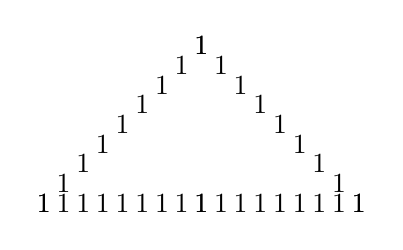
\begin{tikzpicture}
  \drawoddtriangle
\end{tikzpicture}
\end{figure}

Once again, by Pascal's Relation, we get from these facts that
$$\forall 0 \leq i \leq {n - 1}, {{n+1 + i} \choose {1 + i}} \bmod 2 = 0$$

In other words, it forms a decreasing slope of even integers.

By definition, $\pred$ is false for all rows between $n+1$ and $2n$.

Thus, we have $\modrow(2n)=\{1,\underbrace{...}_{n-1},0,\underbrace{...}_{n-1},1\}$

Also, note that ${n+2 \choose 2} \bmod 2 = 1$.

By Pascal's Relation, we get: 
$$\forall 0 \leq i \leq {n-1}, {{n+1+i} \choose i} \mod 2 = 0$$
Thus, we can view ${n+1 \choose 0}$ as recursively spawning a new Pascal Triangle. Thus, from this result, and our assumption (and the symmetry of Pascal's Triangle), $\modrow(2n) = \{1,0,1,0,...1,0,1...0,1,0,1\}$, which implies $\modrow(2n+1) = \{1,1,1...1,1,1,1\} = \modrow(2(2^x-1)+1) = \modrow(2^{x+1}-2+1) =
\modrow(2^{x+1}-1)$.


\end{document}
